% AEJ-Article.tex for AEA last revised 22 June 2011
\documentclass[AEJ]{AEA}

% The mathtime package uses a Times font instead of Computer Modern.
% Uncomment the line below if you wish to use the mathtime package:
%\usepackage[cmbold]{mathtime}
% Note that miktex, by default, configures the mathtime package to use commercial fonts
% which you may not have. If you would like to use mathtime but you are seeing error
% messages about missing fonts (mtex.pfb, mtsy.pfb, or rmtmi.pfb) then please see
% the technical support document at http://www.aeaweb.org/templates/technical_support.pdf
% for instructions on fixing this problem.

% Note: you may use either harvard or natbib (but not both) to provide a wider
% variety of citation commands than latex supports natively. See below.

% Uncomment the next line to use the natbib package with bibtex
%\usepackage{natbib}

% Uncomment the next line to use the harvard package with bibtex
%\usepackage[abbr]{harvard}

% This command determines the leading (vertical space between lines) in draft mode
% with 1.5 corresponding to "double" spacing.
\draftSpacing{1.5}
\usepackage{natbib, graphicx, amssymb, epstopdf}
% To the editor: booktabs is only used for \cmidrule in tables 4 and 6.
\usepackage{enumerate, booktabs}

\renewcommand{\vec}[1]{\ensuremath{\mathbf{#1}}}
\newtheorem{proposition}{Proposition}
\newtheorem{definition}{Definition}

\begin{document}

\title{The Size Distribution of Firms and Industrial Water Pollution \\ A Quantitative Analysis of China}
\shortTitle{FIRM SIZE DISTRIBUTION AND POLLUTION}
\author{Ji Qi, Xin Tang, and Xican Xi\thanks{%
Qi: Chinese Academy for Environmental Planning, Room 709-B BeiKeChuangYe Tower, No.10 Dayangfang, Beiyuan Road, Beijing, China, 100012 (qiji@caep.org.cn); Tang: Center for Economic Development and Research, Economics and Management School, Wuhan University, and International Monetary Fund, 700 19th St NW, Washington D.C., United States, 20431 (zjutangxin@gmail.com); Xi: China Center for Economic Studies, School of Economics, Fudan University, and Shanghai Institute of International Finance and Economics, 600 Guoquan Road, Shanghai, China, 200433 (xicanxi@fudan.edu.cn). We are grateful for the comments from Alexis Anagnostoupolos, Marina Azzimonti, Dong Cao, Juan Carlos Conesa, Berthold Herrendorf, Nicolai Kuminoff, Pietro Peretto, Edward Prescott, Diego Restuccia, Todd Schoellman, V. Kerry Smith, Gustavo Ventura, Jinnan Wang, Daniel Yi Xu, Fang Yu, the editor and three anonymous referees. We also benefited from the comments received from seminars at many institutions. We thank the Ministry of Ecology and Environment for granting us access to the National General Survey of Pollution Sources data. This paper has been screened to ensure that no confidential data are revealed. The results and conclusions in this paper are those of the authors, and do not necessarily reflect the views of the MEE or IMF, its Executive Board, or IMF management. For financial support, Qi acknowledges the National Key R\&D Program of China (2016YFC0207604); and Tang thanks the Key Grant of Ministry of Education of China (16JJD790045).}}
\date{\today}
\pubMonth{Month}
\pubYear{Year}
\pubVolume{Vol}
\pubIssue{Issue}
\JEL{E23, L11, O44, Q52, Q53, Q56}
\Keywords{Firm Size Distribution, Correlated Distortion, Industrial Water Pollution}

\begin{abstract}
    We argue that misallocation across firms amplifies industrial water pollution by distorting the firm size distribution in China. Firm-level data indicate that larger firms are more likely to use clean technology but face higher distortions. In a heterogeneous firms model with an endogenous choice of pollution treatment technologies, we show that distortions that increase with firm-level TFP lower the adoption of clean technology, amplify aggregate pollution intensity, and lower aggregate output. Quantitatively, eliminating these correlated distortions would increase output by 30\% and decrease pollution by 20\%. Meanwhile, environmental regulations have sizable impact on pollution but limited effects on aggregate output.
\end{abstract}

\maketitle

Severe pollution has accompanied China's remarkable economic growth in the past few decades, causing environmental degradation, public health damage and millions of premature deaths.\footnote{\citet{WorldBank_Cost_2007} estimates that the total costs of air and water pollution in China are about 6\% of China's GDP. The health costs of pollution are estimated to be 4\% of GDP in China, the majority of which are associated with premature deaths caused by pollution. See \citet{Vennemoetal:2009} and \citet{ZhengKahn:2013} for reviews of empirical studies on pollution in China.} Understanding the driving forces behind this severe pollution is crucial for designing and evaluating anti-pollution policies. An outstanding question is whether the severe pollution is an inevitable consequence of rapid economic growth, or is it largely exacerbated by policy distortions and/or market inefficiencies.

In this paper, we argue that misallocation across firms amplifies industrial water pollution by distorting the firm size distribution in China. Using nationally representative data on firm production, pollution emissions and pollution treatment technologies, we document two facts on firm size and pollution intensity (pollutants per output) in China. First, large firms have lower pollution intensity than small firms, with an elasticity of $-$0.37 between firm size and pollution intensity for the top five polluting industries (by chemical oxygen demand emissions) in China. Not only do large firms generate  fewer pollutants per output during production, but they are also more likely to use advanced end-of-pipe treatment technologies that require large installation costs. Second, large firms account for a smaller proportion of the total employment in China than in the United States. For the top five polluting industries in China, firms with more than 400 employees account for 20\% of the total employment compared with close to 70\% for the U.S. counterparts. If we take the U.S. economy as a less distorted benchmark, these facts suggest that distortions to firm size distribution could have important environmental consequences in China.

Motivated by these facts, we build a two-sector (polluting and non-polluting) model of heterogeneous firms based on \citet{Lucas:1978b} to evaluate how firm-level distortions affect aggregate output and pollution. The model has the following key features. First, firms in each sector differ in their productivity levels. There is a stand-in household with a continuum of members, and each member draws a sector specific managerial ability from a given distribution. When members choose to be manager, they enter the sector their managerial ability belongs to and the ability determines the TFP of the firm they run. Second, firms differ in pollution intensity as well. As in \citet{CopelandTaylor:1994}, pollution emissions are a by-product of production for firms in the polluting sector. Following Fact 1 above, we assume that generated emissions per output during production is decreasing in firm output. Third, firms have the option to adopt an advanced end-of-pipe treatment technology, which we refer to as clean technology later, after paying a fixed adoption cost. Firms in the polluting sector are subject to environmental regulations such that firms that do not use clean technology face a penalty that takes away a fraction of their profits. As a result, our model predicts that only firms above a certain size threshold would choose the clean technology, which is qualitatively consistent with the fact that large firms are more likely to use clean technology.

Finally, we assume that firms face distortions that increase with their TFP, or \textit{correlated} distortions following the terminology of \citet{RestucciaRogerson:2008}, which are modeled as progressive output taxes.\footnote{\citet{Guneretal:2008} study a closely related type of distortions, namely \textit{size-dependent} distortions, which increase with firm or establishment size (the amount of capital, labor or output). An example is the many labor regulations in Italy, Spain and France that start to bind on firms with more than a certain number of employees. Both correlated and size-dependent distortions lead to a reallocation of resources from high TFP to low TFP firms, and they are essentially equivalent when distortions do not lead to rank reversal defined as more productive firms being smaller [\citet{Hopenhayn:2014}].} We find in our data that firms with higher TFP exhibit substantially higher average products of capital and labor in both the polluting and non-polluting sectors, indicating that more productive firms do face higher distortions [\citet{HsiehKlenow:2009, HsiehKlenow:2014}]. As emphasized by previous studies, such as \citet{RestucciaRogerson:2008} and \citet{HsiehKlenow:2014}, correlated distortions lower both mean firm size and aggregate output, since they limit the operation of productive firms and allow too many unproductive firms to survive and expand. A new insight from our model is that correlated distortions also increase aggregate pollution intensity for two reasons. First, they lower the profits of productive firms which reduce their incentives to adopt the clean technology. Therefore fewer firms adopt clean technology in the equilibrium with correlated distortions. Second, they take production factors away from large productive firms that also have lower pollution intensity, which drives up the average pollution intensity further.

Conventionally, environmental economics decomposes changes in aggregate pollution into three effects: scale (change in aggregate output), composition (reallocation across sectors), and technique (change in sectoral pollution intensity) effects.\footnote{See for example, \citet{GrossmanKrueger:1993}, \citet{CopelandTaylor:2004} and \citet{Levinson:2009} among others.} Our model allows us to assess structurally how distortions affect aggregate pollution through the three channels. Moreover, our model and data allow us to further decompose the technique effect into within sector reallocation across firms and the change caused by the adoption of clean technology.

To discipline our quantitative analysis, we calibrate our model to match the observed pollution intensity, the adoption of clean technology, the correlation between distortions and firm TFP and the firm size distribution in the Chinese data. We map the polluting sector to the top five polluting industries mentioned above, which account for 80\% of the total emissions in the data, and map the non-polluting sector to the rest of the manufacturing sector. We then use the calibrated model to evaluate the effects of two policies: removing correlated distortions from both sectors and strengthening environmental regulations.

Our quantitative results show that removing correlated distortions from both sectors would increase mean firm size by 130\% and aggregate output by 30\%, while lowering the pollution intensity of the polluting sector by 42\%. Since both sectors share similar distributions of firm TFP and distortions in the data, eliminating correlated distortions induces little reallocation across sectors. Therefore, aggregate pollution drops by 23\% because the technique effect dominates the scale effect. About half of the technique effect comes from the reallocation of factors across firms, while the rest is from a 27 percentage points increase in the adoption rate of clean technology. To isolate the importance of the progressiveness of distortions, we solve a version of the model in which the progressive taxes are replaced with flat taxes while holding the total tax revenue constant. Our results show that while the progressiveness of distortions does not imply large output losses, it plays a central role in amplifying aggregate pollution: replacing the progressive taxes with flat taxes would cause a 7\% increase in aggregate output, and a 30\% decrease in aggregate pollution.

In the second experiment, we increase the regulations to the extent that the fraction of firms adopting clean technology is the same as in the first experiment. We find that the policy reduces aggregate pollution by 14\%, but has very limited effect on aggregate output in the long run. Comparing this with the first experiment, we find that tightening environmental regulations improves the resource allocation on the extensive margin of resource allocation by driving small unproductive firms out of the economy. However, the allocation {worsens} on the intensive margin in the sense that among the remaining active firms, the production of medium-sized firms expands more at the expense of that of large firms. In contrast, the removal of correlated distortions improves the allocation on both margins.

Overall, the key message from our findings is that policy distortions and market inefficiencies force developing countries such as China to operate within the production possibility frontier between economic output and environmental quality. Therefore, contrary to a popular belief among some policymakers in developing countries, there is not necessarily a trade-off between economic growth and pollution. Both an increase in output and a reduction in pollution can be attained by reducing policy distortions and market inefficiencies.

%%%%%%%%%%%%%%%%%%%%%%%%%%%%%%%%%%%%%%%%%%%%%%%%%%%%%%%%%%%%%%%%%%%%%%%%%%%%%%%%%%%%%%%%%%%%%%%%%%%%%%%%%%%%%%%%%%%%%%%%%
%                                       STARTING LITERATURE REVIEW
%%%%%%%%%%%%%%%%%%%%%%%%%%%%%%%%%%%%%%%%%%%%%%%%%%%%%%%%%%%%%%%%%%%%%%%%%%%%%%%%%%%%%%%%%%%%%%%%%%%%%%%%%%%%%%%%%%%%%%%%%

\textit{Related Literature.}---This paper is closely related to studies on the aggregate consequences of misallocation across heterogeneous firms. Pioneers in this field such as \citet{Guneretal:2008}, \citet{RestucciaRogerson:2008}, and \citet{HsiehKlenow:2009} establish that firm-level distortions can potentially cause large losses to aggregate output, especially those that correlate with firm size or productivity.\footnote{For more recent works, see \citet{Bartelsmanetal:2013}, \citet{Bhattacharyaetal:2013}, \citet{HsiehKlenow:2014}, \citet{BentoRestuccia:2016}, and \citet{Guneretal:2017}, among others. \citet{RestucciaRogerson:2013}, \citet{Hopenhayn:2014b}, and \citet{RestucciaRogerson:2017} summarize important contributions to the literature.} Our study shows that the impact of firm-level distortions goes beyond aggregate economic output: they cause not only a large decrease in aggregate output, but also a large increase in aggregate pollution. By considering both aggregate output and pollution, our study thus provides a more complete understanding of the consequences of policy distortions given the large costs of pollution in developing countries such as China.

This paper also contributes to a growing literature in environmental economics that emphasizes the importance of firm-level heterogeneity. One line of research uses the heterogeneous firms framework to evaluate specific environmental policies. \citet{LiSun:2015} and \citet{LiShi:2017} compare the welfare effects of emission taxes and standards. Their theoretical findings imply that emission taxes will generally be favored when the dispersion of productivity across firms is large. Relatedly, \citet{TombeWinter:2015} use a heterogeneous firms model calibrated to the U.S. to evaluate the productivity losses from output-based intensity standards. They find that these losses can be large. We differ from this line of research by our focus on how correlated distortions affect aggregate pollution and how they interact with environmental policies.

Another line of research focuses on how international trade affects the environment through resource reallocation across heterogeneous firms. \citet{Cherniwchanetal:2017} provide a comprehensive survey of recent contributions.\footnote{Notable examples include \citet{Martin:2013}, \citet{Cherniwchan:2017}, \citet{BarrowsOllivier:2016}, \citet{Forslidetal:2015} and \citet{ShapiroWalker:2015}. A more detailed comparison between our paper and this line of research can be found in Online Appendix H.} Our paper differs from this literature in two aspects. First, most studies in this literature, with the exception of \citet{ShapiroWalker:2015}, are empirical where models are used primarily to motivate the empirical specification indirectly. Instead, we discipline our general equilibrium model using firm-level data directly in an internally consistent way, and quantitatively assess counterfactual policies using the model. Our quantitative analysis explicitly takes into account the general equilibrium effects of alternative policies, allowing us to investigate novel policy implications that are absent from reduced-form or partial equilibrium analyses. Second, using the firm-level data on treatment technologies, we provide an explanation for the negative correlation between firm size and pollution intensity. It allows us to not only investigate the overall effects of distortions, but also quantify an important channel through which the distortions affect emissions, namely, the adoption of clean technology.

Finally, our results highlight the role of firm size and misallocation for technology adoption in developing countries. As emphasized by \citet{ParentePrescott:1994, ParentePrescott:1999}, an important task in development economics is to understand the slow rate of technology adoption in developing countries. Recent contributions include \citet{Bustos:2011}, who study the role of tariff reductions, and \citet{Acemogluetal:2012}, who focus on taxes and subsidies. Using direct observations on the adoption of pollution treatment technologies by firms, we establish empirically that firm size plays a key role in technology adoption. Our quantitative framework thus allows us to quantify how policy distortions and market inefficiencies that distort firm size would impede technology adoption.

The remainder of the paper proceeds as follows. Section I describes the data sources and empirical findings of this paper. Section II introduces the model and analyzes its property. We calibrate the model in Section III, and perform counterfactual experiments to study the effects of correlated distortions and environmental policies in Section IV. Section V concludes the paper.

\section{Empirical Analysis}

In this section, we describe our empirical findings on the firm-level pollution intensity and the firm size distribution in China. We start by introducing the data sources we use, and then document key facts on pollution intensity, pollution treatment technologies and employment shares across firms of different sizes. In the end, using a simple accounting exercise, we show that firm size distribution plays a quantitatively important role in aggregate pollution intensity.

\subsection{Data Sources}
\label{sec:data_source}

This study draws upon three major data sources: the 2007 National General Survey of Pollution Sources (NGSPS) of China, the 2004 China National Economic Census (CNEC), and the Statistics of U.S. Businesses (SUSB).

\textit{NGSPS.}---The NGSPS was a joint effort of multiple national ministries in China. It covers all of the pollution units from the agricultural, industrial, and domestic sources, as well as facilities for centralized treatment of pollution. In this study, we focus on the {industrial pollution sources}, which consist of businesses generating pollutants from the 39 manufacturing industries. The survey is organized directly by the State Council with data collection and quality control done by specially trained field staff. According to the \textit{Regulation on the National General Survey of Pollution Sources [Decree of the State Council of the People's Republic of China (No. 508)]}, faking data would lead to financial penalties or even lawsuits. Therefore, the dataset is administrative in its nature and is subject to less concerns of systematic under-reporting.\footnote{In fact, uniform under-reporting of emissions by small and large firms will not change the basic conclusions of this paper. Our results will be contaminated only if under-reporting by large firms is more severe than that by small firms, which is less likely in most polluting industries since larger firms are usually inspected more carefully. For instance, many large firms in these industries are identified as \textit{key sources}, and therefore are inspected and monitored by the government routinely and carefully, making it harder for them to fake data during this one-time survey.} While we are not aware of other economic studies that use NGSPS, a number of studies in environmental sciences have used this dataset. See, for example, \citet{Niuetal:2016}, \citet{Qietal:2017} and the references therein. A more detailed description of the dataset can be found in Online Appendix A.

The NGSPS collects information on the emissions of multiple air, water and solid waste pollutants. In this paper, we focus on water pollution mainly because the data are more accurately measured than air pollution.\footnote{After our interview with the field staff, we learned that the difference in data quality was mainly caused by the difference in sampling environment. For water pollution, firms rarely discharge wastewater directly. Instead, the wastewater is first stored in a sedimentation tank to settle heavier solids to the bottom and let lighter materials float. This process creates a stable environment for sampling. For air pollutants, the sampling tube has to be placed in the chimneys, where the environment is much more volatile. Moreover, if firms were to manipulate their instant emissions when the field staff is on-site sampling, the sedimentation process makes it more difficult, since firms would have to clean the tank prior to the on-site visit of the field staff.} Among all the water pollutants, we focus on \textit{chemical oxygen demand} (COD), a major water pollutant that is commonly used to measure water quality. It measures the overall quantity of contaminants that will eventually cause oxygen loss and thus the death of living creatures. We choose COD because a much larger share of firms report positive emissions of COD compared to other pollutants. If we focus on other pollutants, such as hexavalent chromium, we would limit ourselves to a much smaller share of firms that engage in special production processes like leather tanning or pigment manufacturing.\footnote{See Table A.1 in Online Appendix A for the share of firms that report positive emissions for different water pollutants. We would like to stress that many firms do not report emissions of specific pollutants such as cyanidium or chromium simply because they do not use related materials in production. It is not because of under-reporting or other issues related to data quality. In fact, since these pollutants are more hazardous than others, firms that discharge these pollutants are usually monitored more closely.} Moreover, COD emissions are typically highly correlated with the emissions of other pollutants when both are positive.\footnote{In the Paper and Paper Products industry, for example, the correlation between the emissions of COD and $\text{NH}_4^+$ is 0.82 and that between COD and BOD is 0.94.}

The data reveal that industrial water pollutants are typically concentrated in a handful of industries, including COD. In our empirical analysis, we focus on the top five polluting industries by COD emissions, which account for nearly 80\% of all COD emissions from industrial sources. Within narrowly defined manufacturing industries, the NGSPS divides firms into two large groups---\textit{key sources} and \textit{regular sources}. Firms identified as key sources are deemed as more polluting, and therefore are inspected and monitored by the government more carefully. During this census, the field staff also collected extra information on these firms, and the data from these firms were inspected with greater care. Importantly, the key sources include both small and large firms, and the empirical densities of the log output of the key sources resemble the bell shape of those of all firms.\footnote{Please see Online Appendix A.1 for the formal definition of the key sources, and Figure B.1 in Online Appendix B for  the empirical densities of the log output of the key sources.} As a result, when empirically analyzing the relationship of firm size with pollution intensity and treatment technology adoption, we focus on the key sources, which account for more than 90\% of total COD emissions and 80\% of total output from the top five polluting industries (Table \ref{tab:top5summary}). The variables we use are firm's output, the amount of major pollutants generated and emitted, installation costs of pollutant treatment technologies, industry (up to four-digit GB/T4574-2002), ownership classification, and province.

\begin{table}[t]
\footnotesize
\centering
\caption{Statistics of the Top 5 Polluting Industries by COD}
\begin{tabular}{lccccc}
    \hline \hline
                                       & Paper & Food & Textiles  & Chemicals & Beverages  \\
    \hline
    \% in Total COD Emission           & 33.4  & 15.1 & 14.0 & 10.4 & 4.27  \\
    \% of Emissions by Key Sources     & 99.6  & 91.8 & 91.1 & 99.7 & 65.1  \\
    \% of Production by Key Sources    & 87.2  & 69.3 & 48.3 & 98.6 & 88.1  \\
    \hline
\end{tabular}
\begin{tablenotes}[Sources]
     NGSPS. The acronyms respectively refer to (with the two-digit GB/T4547-2002 classification code in parentheses): Paper and Paper Products (C22), Processing of Food from Agricultural Products (C13), Textiles (C17), Raw Chemical Materials and Chemical Products (C26), and Beverages (C15).
\end{tablenotes}
\label{tab:top5summary}
\end{table}

\textit{CNEC.}---The CNEC was conducted by the National Bureau of Statistics in China. It was designed to cover {all} businesses that undertake economic activities in the secondary and tertiary industries in China. We use observations that belong to the manufacturing sector. The variables we use are firm's output, labor compensation, book value of capital stock, number of employees, industry (up to four-digit GB/T4574-2002), ownership classification, and province.\footnote{A widely used firm-level dataset in China is the Annual Surveys of Industrial Firms (ASIF). We use CNEC instead of ASIF because that ASIF does not have information on non-state firms with sales below 5 million CNY, which are crucial for our analysis. If we used the 2004 ASIP, we would have missed 29\% of the employment and 80\% of the firms.}

\textit{SUSB.}---The SUSB from the U.S. Census Bureau, is an annual series that provides national and subnational data on the distribution of economic activities by firm size and industry. We use the data on total employment by firm size and industry from 2004.

\subsection{Firm Size and Pollution Intensity}

\begin{figure}[t]
\caption{Firm Size and Pollution Intensity}
\label{fig:codscatter}
    \begin{center}
    \includegraphics[width=0.40\textwidth]{./Figures/pooled_intensity_size.pdf}
    \end{center}
    \begin{figurenotes}[Source]
        NGSPS.
    \end{figurenotes}
    \begin{figurenotes}
        The line is the least square fit. Residuals after controlling for the covariates are plotted.
    \end{figurenotes}
\end{figure}

\textit{Firm Size and Pollution Intensity.---}To examine the statistical relationship between pollution intensity and firm size for the polluting sectors in China, we run the following regression using data on firms identified as key sources in the top five polluting industries:
\begin{equation}
    \log (\text{COD}_i) = \underset{(0.17)}{-3.75} + \underset{(0.01)}{0.63} \times \log (\text{Output}_i) + \vec{X} \vec{\gamma} + \varepsilon_i,
\label{eq:poolols}
\end{equation}
where $\vec{X} = \{\vec{X_s}, \vec{X_p}, \vec{X_o}\}$ refers to the dummy variables for two-digit industry, province and ownership respectively. The estimates are all statistically significant at 0.1\% level, with standard errors reported in the parentheses below the estimates.

These estimates imply that as a firm's output increases by 1\%, its COD emissions would on average increase by only 0.63\%. We define pollution intensity as COD emissions per unit of output. Then the above estimates imply an elasticity of $-$0.37 between firm-level pollution intensity and output. That is, other things equal, a 1\% increase in firm output is associated with a 0.37\% decrease in pollution intensity. Figure \ref{fig:codscatter} visualizes this negative relationship, where the residuals from regressing intensity and output on the dummies are plotted to remove the influences of other covariates. The estimation has an $R^2$ of 0.41, suggesting that nearly half of the variations in COD emissions can be explained by the variations in firm output and in the three sets of dummies.\footnote{We also tried other econometric specifications, and found similar negative correlations between pollution intensity and firm size. For instance, we estimated versions of Equation (\ref{eq:poolols}) for each industry and with robust standard errors clustered by provinces. Please see Online Appendix C for more information.} We would also like to point out that the coefficient of the dummy on whether a firm is state-owned or not, is statistically insignificant. As a result, we do not distinguish between whether a firm is state-owned or not in our later analysis.

\textit{The Role of End-of-Pipe Treatment Technologies.---}An important question is, why do larger firms have lower pollution intensity? To answer this question, we exploit the detailed information on the end-of-pipe wastewater treatment technologies that firms use in the NGSPS. The NGSPS groups wastewater treatment technologies into five categories: physical, chemical, physio-chemical, biological, and {combined} technologies. In the subsequent analysis, we drop {physio-chemical} technology because fewer than 0.5\% of the firms adopt this type of technology. In addition, because {combined} technology looks very similar to biological technology for all the technical aspects we are interested in, we group them with {biological} technology.\footnote{Examples of the technologies attributed to these three base categories include filtering, centrifuging, precipitation, and separation (physical); oxidation reduction and neutralization (chemical); and aerobic biological treatment and activated sludge processes (biological). Broadly speaking, physical technology corresponds to the \textit{Preliminary} and \textit{Primary} treatment in the U.S., while chemical and biological technologies correspond to the \textit{Secondary} and \textit{Tertiary} treatment.} In sum, we are left with three broad categories of technologies.

To illustrate the difference in technology adoption by firms of different sizes, we use the Paper and Paper Products industry as an example. By focusing on one specific industry, we abstract from the potential heterogeneity in production processes across industries. Table \ref{tab:techeffi} shows the mean abatement efficiency, median installation costs, and median output of firms that adopt these technologies, where the {abatement efficiency} is defined as one minus the ratio of {emitted COD} to {generated COD}.
\begin{table}[t]
\footnotesize
\centering
\caption{Firm Size and Treatment Technologies}
\begin{tabular}{lcccc}
    \hline \hline
    Technology  & Mean Efficiency & Adoption Rate & Median Costs & Median Output \\
    \hline
    Physical    & 63.37\%         & 25.89\%       & 100          & 100                       \\
    Chemical    & 74.96\%         & 33.64\%       & 308          & 219                       \\
    Biological  & 80.90\%         & 38.60\%       & 923          & 500                       \\
    \hline
\end{tabular}
\label{tab:techeffi}
\begin{tablenotes}[Source]
     NGSPS.
\end{tablenotes}
\begin{tablenotes}
     The numbers reported are for the Paper and Paper Products (C22) industry. Abatement efficiency is defined as $1 - \text{COD Emitted}/\text{COD Generated}$. The median installation costs of physical technologies and median output of firms that adopt them are normalized to 100.
\end{tablenotes}
\end{table}
We find that for each 100 tons of COD generated, firms with biological technology on average emit 19.1 tons of COD, compared to 36.6 tons for firms with physical technology. Meanwhile, the median installation costs of biological technology are 8 times higher than those of physical technology. In addition, the median output of the firms using biological technology are 4 times higher than those of firms with physical technology. These evidence points to increasing returns to scale in the adoption of cleaner technologies. As a result, small firms lack the profit margins needed to take advantage of these increasing returns to scale, while large firms are more likely to adopt cleaner technologies.

To see the statistical relationship between firm size and technology adoption, we pool all five polluting industries together and estimate a linear probability model of treatment technology adoption with the same set of covariates as in Equation (\ref{eq:poolols}):
\begin{equation*}
    y_i = \underset{(0.04)}{0.23} + \underset{(0.001)}{0.05} \times \log (\text{Output}_i) + \vec{X} \vec{\gamma} + \epsilon_i,
\end{equation*}
where $y_i$ is a dummy variable which equals to 1 when a firm uses biological technology. The estimates show that doubling a firm's output leads to a 5 percentage points increase in the adoption rate of biological technology. This confirms our previous finding with the paper industry that larger firms are more likely to use cleaner technologies.

\textit{Emissions Generated during Production.---}Another reason behind the negative correlation between pollution intensity and firm size is that large firms also generate less COD per output during the production stage. In particular, if we divide our sample into two groups according to whether a firm is using biological technology or not and repeat regression (\ref{eq:poolols}) again, we find significantly negative correlations between COD per output and firm size within each group:
\begin{align}
\label{eq:poolols_biological}
    \text{Biological:} \quad \log (\text{COD}_i) &= \underset{(0.20)}{-4.37} + \underset{(0.01)}{0.67} \times \log (\text{Output}_i) + \vec{X} \vec{\gamma} + \varepsilon_i, \\
\label{eq:poolols_others}
    \text{Others:} \quad \log (\text{COD}_i) &= \underset{(0.31)}{-3.41} + \underset{(0.01)}{0.64} \times \log (\text{Output}_i) + \vec{X} \vec{\gamma} + X_e \gamma_e + \varepsilon_i,
\end{align}
where $X_e$ is the dummy for chemical equipment.\footnote{In our model and quantitative analysis below, we assume two types of treatment technologies. This is why we divide firms into two groups here. Running regression (\ref{eq:poolols}) separately for firms using physical and chemical equipments yield similarly significantly negative correlations between COD per output and firm size for each technology. Online Appendix C.3 reports the results in detail.}

Such within group negative correlations could be because that larger firms use cleaner or fewer inputs to produce the same amount of output. For one example, the paper pulp industry uses two different types of inputs: bagasse and wood. According to the \textit{Handbook of Emission Coefficients} by the Chinese Academy of Sciences, bagasse, which is mostly used by firms with an annual production of less than 100 kilotons, generates 140--180 kg of COD per ton of output, while wood, which is mostly used by firms with an annual production of more than 100 kilotons, generates 30--55 kg of COD per ton of output. As another example, \citet{Bloometal:2010} find that better managed firms use less energy to produce the same amount of output in the U.K. Unfortunately, we cannot test these hypotheses directly using our data. Instead, we focus on firms' decisions to adopt treatment technologies, and model the emissions reduction during the production stage in a reduced-form way based on Equations (\ref{eq:poolols_biological}) and (\ref{eq:poolols_others}).

\subsection{Firm Size Distribution and Aggregate Pollution Intensity}

The negative correlation between pollution intensity and firm size suggests that firm size distribution plays a potentially important role in aggregate pollution intensity. To illustrate this point, we document facts on the firm size distributions in China and in the U.S., and compute the change in the aggregate pollution intensity if the firm size distribution for the top five polluting industries in China were replaced with that in the U.S. We choose the U.S. as the benchmark because it is a relatively less distorted economy; and China and the U.S. are both large economies with a complete set of industries so that we can find comparable industries in both economies.\footnote{It is a commonly used strategy in the macro-development literature to take the U.S. economy as an undistorted benchmark. See \citet{Guneretal:2008}, \citet{HsiehKlenow:2009, HsiehKlenow:2014}, \citet{Bartelsmanetal:2013} and \citet{AdamopoulosRestuccia:2014}, among others.}

Since the SUSB does not report information on output, we focus on the shares of employment accounted for by firms of different sizes, since firm-level employment is strongly correlated with output. We use the \textit{International Standard Industrial Classification of All Economic Activities, Revision 3.1} (ISIC Rev. 3.1) published by the United Nations to bridge the different industrial classification systems adopted by China (GB/T4574-2002) and the U.S. (NAICS 2002). Specifically, we use the crosswalks of GB/2002 at the four-digit level and those of NAICS/2002 at the six-digit level to the ISIC Rev. 3.1 issued respectively by the National Bureau of Statistics of China and the U.S. Census Bureau, respectively.
\begin{figure}[t]
    \begin{center}
    \includegraphics[width=0.45\textwidth]{./Figures/poolES_R_1.pdf}
    \includegraphics[width=0.45\textwidth]{./Figures/allES_R_1.pdf}
    \caption{Employment Distributions}
    \begin{figurenotes}[Sources]
        CNEC and SUSB.
    \end{figurenotes}
    \label{fig:es}
    \end{center}
\end{figure}

The left panel of Figure \ref{fig:es} depicts the firm size distribution for the top five polluting industries pooled together. We find that approximately 70\% of employment in the U.S. is accounted for by firms with 400+ employees, while in China the number is only 20\%.\footnote{In Online Appendix E, we compare the firm size distributions between China and the U.S. for each individual polluting industry. We find that while there is substantial heterogeneity across individual industries, large firms in China account for a much smaller employment shares than those in the U.S. for all five industries.}
Compared with the U.S., a much larger share of production is carried out by small and medium-sized firms in China. From the right panel of Figure \ref{fig:es}, we find a similar pattern for the whole manufacturing sector.

\textit{An Accounting Exercise.---}To see the potential importance of firm size distribution, we conduct the following accounting exercise. For the top five polluting industries in China, we fix the total output and  the estimated firm size--pollution intensity relationship, and replace the firm size distributions with those in the U.S. Then we compute the resulting average pollution intensity for these polluting industries pooled together. This simple exercise is complicated by the fact that the NGSPS reports firm-level output instead of number of employees. Therefore, we construct an employment--output relationship from a linear regression using the CNEC data.\footnote{There are different methods to construct the employment--output relationship using the CNEC data, but all of them provide similar results. See Online Appendix F for details.}

We find that the average pollution intensity for the pooled top five polluting industries drops by 33\%, when the firm size distributions in these industries are changed to those in the U.S. This would cause a 25\% decrease in the average pollution intensity for the whole manufacturing sector if we leave other manufacturing industries untouched. Admittedly a crude approximation, this exercise nevertheless shows that distortions to firm size distribution could potentially have a large impact on aggregate pollution intensity.

\section{The Model}

The above accounting exercise is illuminating but has several limitations. First, the firm size distribution is mechanically changed to that in the U.S. Although the U.S. economy is often taken as a benchmark in the development literature, it is unclear whether the differences in firm size distribution between China and the U.S. are mainly caused by distortions or by some other factors. Second, the accounting exercise captures the technique effect only, while distortions may operate through the scale and composition effects as well. Third, the relationship between firm size and emissions intensity is taken as exogenous in the accounting exercise. However, distortions to firm size may also influence firm's incentive to adopt different treatment technologies, which endogenizes the firm size--intensity relationship.

To address these issues, we build a two-sector (polluting and non-polluting) model of heterogeneous firms based on the classic \citet{Lucas:1978b} span-of-control model.\footnote{A widely used alternative  in the misallocation literature is the closed-economy version of the \citet{Melitz:2003} model. \citet{HsiehKlenow:2009} establish that these two frameworks are isomorphic for the effects of misallocation on aggregate output when the number of firms is fixed. In Appendix G.3, we show the qualitative equivalence between the two families of models as well.} The model features heterogeneity in firm productivity in both sectors, heterogeneity in pollution intensity and an endogenous choice of pollution treatment technologies in the polluting sector. Motivated by the data, firms in both sectors are subject to correlated distortions [\citet{RestucciaRogerson:2008}] in the form of progressive output taxes. %Throughout, we refer to the sectors as polluting and non-polluting, and technologies as dirty and clean.
In the context of our model, the polluting sector is mapped to the top five polluting industries and the non-polluting sector to the rest of the manufacturing sector, while clean and dirty technologies are interpreted as biological and other (physical plus chemical) equipments as specified in Section I.B.

\subsection{Setup}

We assume that the products of the two sectors in the model economy are perfect substitutes to each other.\footnote{In Online Appendix J, we consider the case in which the final good is a CES aggregation of the goods produced in the two sectors, and conduct counterfactual experiments under different values of the elasticity of substitution in the CES function. For the counterfactual experiments we discuss in the main text, the quantitative results in the CES cases are similar to those in the perfect substitute case, largely because the experiments induce very limited reallocation between sectors.} The polluting sector generates emissions as a by-product of production as in \citet{CopelandTaylor:1994}, while the non-polluting sector does not. The top five polluting industries (henceforth the polluting sector) account for nearly 80\% of total industrial COD emissions and 20\% of total industrial output, with the rest accounted for by the non-polluting sector. Firms in both sectors behave competitively.

\textit{Household.}---There is a representative household with a continuum of members that maximizes the life-time utility $\sum_{t=0}^{\infty} \beta^t U(C_t)$, where $C_t$ is the consumption at time $t$ and $\beta$ is the discount factor.

A fraction $\mu$ of the members are endowed with managerial talent that can be used in the polluting sector, drawn from a distribution with cumulative distribution function (CDF) $G^{d}(z)$, where the superscript $d$ refers to the polluting sector. Meanwhile, a fraction $1-\mu$ of the members are endowed with managerial talent for the non-polluting sector with CDF $G^{c}(z)$, with the superscript $c$ referring to the non-polluting sector. The support for both distributions are $Z \triangleq [0,\overline{z}]$. We assume that $z$ is fixed once drawn. Household members face an occupational choice between {worker} and {manager}. A worker supplies one unit of labor inelastically in exchange for wage income, and is perfectly mobile between sectors, while a manager in each sector runs a neoclassical firm and earns profits. As we see in Figure \ref{fig:es}, the firm size distributions in the polluting sector and the whole manufacturing sector are almost identical. Based on this observation, we assume that $G^{d}(z) = G^{c}(z) \triangleq G(z)$ from now on.

In addition, we assume that the household owns all the firms and capital in this economy. The goods produced in the non-polluting sector are taken as the numeraire. With perfect substitution between goods, the price of the polluting sector product is also 1. $R$ and $W$ are the capital rental price and wage rate, respectively.

\textit{Firms.}---The production functions in the two sectors take the same form. Production requires managerial talent $z$, capital $k$, and labor $l$. For a firm run by a manager with managerial talent $z$, its output is
\begin{equation*}
    y = F(z,k,l) = z^{1-\gamma} (k^{\alpha}l^{1-\alpha})^{\gamma},
\end{equation*}
where $0<\gamma<1$ is the span-of-control parameter, which governs the returns to scale at the firm level. Due to diminishing returns to scale at the firm level, a non-degenerate distribution of firm size can be supported, and firms earn positive profits as the payment to managerial talent $z$. As is typically the case with studies that follow \citet{Lucas:1978b}, managerial talent $z$ is the only source of firm-level TFP in this model. In what follows, we also refer to $z$ as firm-level TFP.

In the non-polluting sector, firms do not discharge pollutants and are not subject to environmental regulations. In the polluting sector, pollutants $e$ are generated as a by-product of production. Total emissions $e = \mathcal{E}(j,y)$ depend on the amount of output $y$, and the pollution treatment technology firms use, with $j = 1$ refers to the clean technology and $j = 0$ the dirty technology. Based on the empirical findings from Section I, we assume that
\begin{equation}
\label{eq:intensity_size}
    \log\left(\frac{e}{y}\right) = \psi_0^{j}+ \psi_1^{j} \log y, \quad j = 0,1,
\end{equation}
where $\psi_1^{j}<0$. This formulation indicates that larger firms emit fewer pollutants per unit of output, which is consistent with our empirical findings in Section I.B.

Adopting the clean technology incurs fixed cost $R k_E$. We assume that the environmental authority punishes firms for using the dirty technology. Similar in spirit to \citet{ShapiroWalker:2015}, we model environmental regulations in a parsimonious way as a penalty which equals to a proportion $\xi$ of the firm's profits. The penalty is later redistributed to the household as lump-sum transfers.\footnote{In practice, China employs both economic incentives and command-and-control instruments in its current industrial pollution management and control system. A powerful tool used by the Chinese government is to randomly audit and then shut down firms that do not comply with environmental regulations for a certain period of time, which would cost these firms a fraction of their profits. See Trevor Nace, ``China shuts down tens of thousands of factories in widespread pollution crackdown,'' Forbes, October 24th 2017, for an anecdotal example.  We present a short summary of China's current environmental regulations based on \citet{Lin:2013} in Online Appendix D.3.} Therefore, the central trade-off in a firm's technology choice is weighing the adoption cost $R k_E$ against the profit losses from environmental penalties. To the extent that firm's profits increase with firm size, we implicitly capture the size-dependency of environmental regulations, in the sense that larger firms are usually monitored and inspected more closely. A key prediction from these assumptions is that, only firms above a certain size threshold would choose the clean technology, which is qualitatively consistent with our empirical findings on technology adoption in Section I.B.\footnote{In Online Appendix D.2, we provide further evidence that the ratio of a firm's expenditures on treatment technology to firm output decreases with firm size, which supports the fixed cost assumption.}

\textit{Correlated Distortions.---}Finally, we introduce the correlated distortions at the firm level to both sectors as implicit progressive output taxes which increase with a firm's productivity levels. The functional form of the tax is:
\begin{equation}
    \tau^i_z = \max \left\{ 0, 1 - \phi_0^i z^{\phi_1^i} \right\}, i=c,d,
\label{eq:tax}
\end{equation}
where the parameter $\phi_0^i$ determines the mean level of the taxes, and the parameter $\phi_1^i$ determines the progressivity of the taxes. When $\phi_1^i<0$, the tax rates are increasing in firm TFP $z$, and the progressivity of the taxes is decreasing in the value of $\phi_1^i$.\footnote{This tax function has a long history in macro-public finance literature, which dates back to at least \citet{Benabou:2002}. We thank a referee for pointing this out. Recent studies that use this function include \citet{HsiehKlenow:2014}, \citet{BentoRestuccia:2016} and \citet{Guneretal:2017}. In Online Appendix D.1, we discuss distortions that take more general forms, and present empirical evidence in support of this specific form. Figure D.2 in Online Appendix D provides an illustration of this tax function.}

The tax function (\ref{eq:tax}) is consistent with the positive relationship between firm TFP and average product of factors we find in the CNEC data. This can be seen from Figure \ref{fig:apf}, which depicts the geometric average of the average product of labor and capital $(y/k)^\alpha(y/l)^{1-\alpha}$ against firm TFP $z$ for both the polluting and non-polluting sectors.\footnote{To estimate firm TFP and average product of factors, we need to assign the values to the parameter that determines the income share of capital, $\alpha$, and the span-of-control parameter, $\gamma$. We take these values from our calibration in Section III, which implies that $\alpha = \text{0.54}$ and $\gamma = \text{0.93}$. The positive relationship between firm TFP and average product of factors, however, holds for a wide range of values for $\alpha$ and $\gamma$, in addition to the values used here. Moreover, similar patterns are also observed in other countries. For instance, \citet{HsiehKlenow:2014} find a strong and positive relationship between firm TFP and average product of factors in India and Mexico, while \citet{BentoRestuccia:2016} document similar patterns for dozens of developing countries.} It can also be seen that the relationships between the average product of factors and firm TFP in these two sectors share very similar slopes. Based on this observation, we assume $\tau^c_z = \tau^d_z \triangleq \tau_z$ from now on.

The firm-level distortions $\tau_z$ are meant to capture a variety of policies and institutions that reallocate production factors from large productive to small unproductive firms, following the \emph{indirect} approach in the misallocation literature [\citet{RestucciaRogerson:2013,RestucciaRogerson:2017}]. These policies and institutions include size-dependent taxes and subsidies that favor small firms, imperfect tax enforcement that induces tax evasion among small firms, financial constraints and contractual frictions that impede the growth of productive firms [\citet{CooleyQuadrini:2001}, \citet{ClementiHopenhayn:2006} and \citet{Akcigitetal:2018}] and local protectionism and internal trade barriers that disproportionately affect large productive firms [\citet{Eberhardtetal:2016} and \citet{TombeZhu:2015}]. While it is of great policy interest to study specific policies and institutions underlying $\tau_z$, we leave this important task to future work.

\begin{figure}[t]
    \begin{center}
    \includegraphics[width=0.45\textwidth]{./Figures/apf_pol_weight.pdf}
    \includegraphics[width=0.45\textwidth]{./Figures/apf_npol_weight.pdf}
    \caption{Average Product of Factors versus Firm Productivity in the Cross-Section}
    \begin{figurenotes}[Source]
        CNEC.
    \end{figurenotes}
    \begin{figurenotes}
        Both variables have been normalized to reflect the relative values to the sectoral averages, which are similar across sectors.
    \end{figurenotes}
    \label{fig:apf}
    \end{center}
\end{figure}

\subsection{Firm's Profit Maximization Problem}

Firms in the non-polluting sector solve the standard profit maximization problem:
\begin{equation*}
    \pi^c(z) = \max_{k,l} \left\{ (1-\tau_z) z^{1-\gamma}(k^{\alpha}l^{1-\alpha})^{\gamma} - Wl - Rk \right\},
\end{equation*}
where the superscript $c$ refers to the non-polluting sector.

Firms in the polluting sector choose first the optimal treatment technology and then the optimal production plan. The profit function $\pi^d(z)$ is the envelope of the profits when using the dirty technology $\pi_0^d(z)$ and clean technology $\pi_1^d(z)$:
\begin{equation*}
    \pi^d(z) = \max \left\{ \pi_0^d(z), \pi_1^d(z) \right\},
\end{equation*}
where the superscript $d$ refers to the polluting sector, and the subscripts denote the treatment technologies. Firms using the clean technology are not subject to environmental penalties, hence the profit $\pi_1^d(z)$ is:
\begin{equation*}
    \pi_1^d(z) = \max_{k,l} \left\{ (1-\tau_z) z^{1-\gamma} (k^{\alpha} l^{1-\alpha})^{\gamma} - Wl - R (k+k_E) \right\}.
\end{equation*}
However, when a firm chooses the dirty technology, it will be punished by the environmental authority, and loses a fraction $\xi$ of its gross profit. The net profit $\pi_0^d(z)$ is thus:
\begin{equation*}
    \pi_0^d(z) = \max_{k,l} \left\{ \left( 1 - \xi \right)
        \left[ (1-\tau_z) z^{1-\gamma} (k^{\alpha} l^{1-\alpha})^{\gamma} - Wl - Rk \right] \right\}.
\end{equation*}

The firm's problem implies that there exists a firm size threshold $\tilde{l}^d$ above which firm will choose the clean technology, which is consistent with our empirical finding that larger firms are more likely to use the clean technology. This can be seen by comparing the potential profits from using clean versus dirty technology:
\begin{equation*}
    \pi_1^d(z) - \pi_0^d(z)  = \frac{\xi(1-\gamma)}{(1-\alpha)\gamma}Wl^d(z) - Rk_E.
\end{equation*}
When $1-\gamma+\phi_1 > 0$, which is satisfied given our calibrated values for $\gamma$ and $\phi_1$, $\pi_i^d(z)$ and $l^d(z)$ are both increasing $z$. Then, as we show in Lemma 2 of Online Appendix G.1, there exists a threshold $\tilde{z}_d$ (hence $\tilde{l}^d$) such that only firms with TFP higher than $\tilde{z}_d$ would choose clean technology. There also exist two thresholds $\hat{z}_i, i=c,d,$ such that in sector $i$, only members with $z > \hat{z}_i$ choose to be managers.

\subsection{Stationary Equilibrium}

In this section, we close the model by specifying the household's optimization problem, and then define the stationary equilibrium.

The household solves the standard consumption-saving problem:
\begin{align}
\label{eq:household}
    & \max_{C_t, K_{t+1}} \sum_{t=0}^{\infty} \beta^t U(C_t) \\
    & s.t.  \nonumber \\
    & \qquad C_t + K_{t+1} - (1-\delta)K_t = I_t, \nonumber
\end{align}
where $K_t$ is aggregate capital, $\delta$ is depreciation rate and $I_t$ is household income, which we specify in detail shortly.\footnote{Here we do not explicitly model the household's preference over water quality. Adding water quality to the household's utility function will not change the firm's choices in a competitive equilibrium, as no individual household member has any control over the aggregate environmental quality. However, if we study the social planner's problem instead, the household's preference over water quality will become a major modeling choice.} The solution to (\ref{eq:household}) is the standard intertemporal Euler equation:
\begin{equation*}
    U'(C_t) = \beta U'(C_{t+1})(1+R_{t+1}-\delta),
\end{equation*}
which pins down the equilibrium interest rate.

Household income $I_t$ comes from three sources: wage and interest income, firms' profits, and lump-sum transfers from taxes $\tau_z$ and environmental penalties $\xi$. If we let $T$ denote the transfers, then household income is\footnote{We have implicitly assumed that firms using clean and dirty technologies coexist in the equilibrium, meaning that $\hat{z}_d<\tilde{z}_d$. This is also the case in our quantitative exercises later.}
\begin{align*}
    I &= R K + W [\mu G(\hat{z}_d)+(1-\mu)G(\hat{z}_c)] + T \\
      & \qquad + \mu\left[\int_{\hat{z}_d}^{\tilde{z}_d} \pi^d_0(z) dG(z) + \int_{\tilde{z}_d}^{\overline{z}} \pi^d_1(z)dG(z)\right] + (1-\mu)\int_{\hat{z}_c}^{\overline{z}}\pi^c(z)dG(z),
\end{align*}
where the transfers $T$ are given by
\begin{equation*}
    T = \mu\xi\int_{\hat{z}_d}^{\tilde{z}_d}\pi^d(z)dG(z) + \tau_z\left[\mu \int_{\hat{z}_d}^{\overline{z}} \pi^d(z) dG(z) + (1-\mu)\int_{\hat{z}_c}^{\overline{z}} \pi^c(z) dG(z) \right].
\end{equation*}

Let $Y$ be aggregate output and $E$ be aggregate pollution, then the stationary equilibrium of the model is defined as follows.
\begin{definition}
\label{def:ge}
cA stationary equilibrium of the model consists of prices $\{W, R \}$, allocations $\{C, K, Y \}$, firms' policy functions $\{k^j(z),l^j(z),y^j(z),\pi^j(z)\}, j = c,d$, thresholds for household's occupational choices $\{\hat{z}_c, \hat{z}_d\}$ and polluting firms' technology adoption $\tilde{z}_d$, as well as aggregate pollution $E$, such that:
\begin{enumerate}[(i)]
    \item
    Given factor prices $\{W, R\}$, $\{C, K, \hat{z}_c, \hat{z}_d\}$ solve the household's optimization problem;
    \item
    Given factor prices $\{W, R\}$, $\{k^j(z),l^j(z),y^j(z),\pi^j(z)\}$, $j = c,d$, and $\tilde{z}_d$ solve the firms' optimization problems;
    \item
    Factor prices $\{W, R\}$ clear all markets:
    \begin{itemize}
        \item
        Labor Market:
        \begin{equation*}
            \mu G(\hat{z}_d) + (1-\mu) G(\hat{z}_c) = \mu \int_{\hat{z}_d}^{\overline{z}} l^d(z)dG(z) + (1-\mu)\int_{\hat{z}_c}^{\overline{z}} l^c(z)dG(z),
        \end{equation*}
        \item
        Capital Market:
        \begin{equation*}
            K = \mu \left[\int_{\hat{z}_d}^{\overline{z}} k^d(z)dG(z) + k_E [G(\overline{z})-G(\tilde{z}_d)]\right] + (1-\mu)\int_{\hat{z}_c}^{\overline{z}} k^c(z)dG(z),
        \end{equation*}
        \item
        Product Market (Walras' Law):
        \begin{equation*}
            C + K - (1-\delta)K = \mu \int_{\hat{z}_d}^{\overline{z}} y^d(z)dG(z) + (1-\mu)\int_{\hat{z}_c}^{\overline{z}} y^c(z)dG(z);
        \end{equation*}
    \end{itemize}
    \item
    Aggregate Pollution:
    \begin{equation*}
        E = \mu\left[\int_{\hat{z}_d}^{\tilde{z}_d} e\left(0,y^d(z)\right)dG(z) + \int_{\tilde{z}_d}^{\overline{z}} e\left(1,y^d(z)\right) dG(z)\right].
    \end{equation*}
\end{enumerate}
\end{definition}
\noindent The algorithm to compute the stationary equilibrium is sketched in Online Appendix I.

\subsection{Correlated Distortions, Technology Adoption, and Aggregate Pollution}
\label{sec:analytical}

In this section, we show qualitatively how correlated distortions modeled as Equation (\ref{eq:tax}) affect the adoption of clean technology across firms and the aggregate pollution. First, we show that correlated distortions have a negative impact on firms' incentives to adopt the clean technology. Second, using a simplified one-sector model with a fixed number of firms and exogenous firm-level pollution intensity, we characterize the conditions under which correlated distortions lead to higher aggregate pollution. The core trade-off here is between the scale and technique effects, because removing the correlated distortions generally brings a decrease in average pollution intensity but an increase in aggregate output. All the proofs and related analytical results can be found in Appendices G.1 and G.2.

\textit{Technology Adoption.---}Proposition \ref{prop:friction} shows that correlated distortions discourage firms from adopting of clean technology, especially those with medium levels of TFP.
\begin{proposition}
\label{prop:friction}
When $1-\gamma+\phi_1>0$, a firm chooses to install clean technology only when its productivity is higher than a threshold. Moreover, the threshold when the firm faces distortions $\tilde{z}_f$ is higher than that when the firm is not subject to any distortions $\tilde{z}_n$.
\end{proposition}

\begin{figure}[t]
\begin{center}
    \includegraphics[width=0.60\textwidth]{./Figures/prod_tax_effect.pdf}
    \caption{Correlated Distortions and Treatment Technologies}
    \label{fig:constantp}
    \begin{figurenotes}
        There are four profit functions in the figure, $\pi_0^n, \pi_0^f, \pi_1^n$, and $\pi_1^f$. The superscripts $n$ and $f$ denote whether firms face correlated distortions in the economy or not, and the subscripts $0$ and $1$ denote whether firms choose the dirty or clean technology, respectively.
    \end{figurenotes}
\end{center}
\end{figure}
\noindent Figure \ref{fig:constantp} illustrates the intuition behind Proposition \ref{prop:friction}. Recall that while the adoption cost $Rk_E$ is independent of $z$, the penalty for not using the clean technology $\xi \pi_0(z)$ is increasing in $z$. Therefore, the adoption of the clean technology pays off for firms with higher $z$. On the other hand, the elasticity of profits to productivity $z$ is $1-\gamma$ when there are no distortions, and is $1-\gamma+\phi_1$ when distortions exist. Since $\phi_1 < 0$, the slope of the profit functions are flatter, and the threshold where firms switch technologies is higher when they face distortions. As a result, while firms with TFP in the range $[\tilde{z}_n, \tilde{z}_f]$ would choose the clean technology when they are not subject to distortions, they will choose the dirty technology instead when distortions exist.\footnote{Of course, when the correlated distortions apply to all firms in the economy, they would affect the equilibrium wage $W$ and hence $\tilde{z}_f$ in equilibrium. We find later in our quantitative analysis that $\tilde{z}_f > \tilde{z}_n$ even when general equilibrium effects are considered.}

\textit{Aggregate Pollution.---}To derive a closed-form expression for the relationship between correlated distortions and aggregate pollution, we build a simplified one-sector model that abstracts from endogenous occupation choice and treatment technology choice. This complements our analysis in Proposition \ref{prop:friction}, which focuses on how distortions affect firms' decision in that the general equilibrium effects are captured. Proposition \ref{prop:agge} summarizes our main findings.
\begin{proposition}
\label{prop:agge}
In the simplified model, there exists a threshold
\begin{equation*}
    \hat{\phi}_1 = \frac{\psi_1(1-\gamma)}{1-\gamma(1+\psi_1)},
\end{equation*}
such that $E$ is increasing in $\phi_1$ when $\phi_1 < \hat{\phi}_1$ and decreasing when $\phi_1 \geq \hat{\phi}_1$.
\end{proposition}

Proposition \ref{prop:agge} says that the relationship between $E$ and the progressivity of the distortions $|\phi_1|$ is inverted-U shaped with the turning point $|\hat{\phi}_1|$ increasing in the elasticity of emission intensity to output $|\psi_1|$.\footnote{Since $\phi_1$ and $\psi_1$ are both negative, the progressivity and elasticity are stronger when $|\phi_1|$ and $|\psi_1|$ are larger, meaning that the raw values $\phi_1$ and $\psi_1$ are smaller.} Because correlated distortions generally decreases the total output while increasing the average pollution intensity, the intuition behind Proposition \ref{prop:agge} is a race between the scale and technique effects. In particular, the scale effect is larger when the progressivity of the distortions is stronger (a smaller negative $\phi_1$), while the technique effect is larger when the elasticity of emission intensity to output is larger (a smaller negative $\psi_1<0$). As a result, when $|\phi_1|$ is not too large relative to $|\psi_1|$, the technique effect dominates. Hence an increase in $\phi_1$ (which means a decrease in the progressivity) causes higher aggregate pollution $E$. Otherwise, the scale effect dominates, and an increase in $\phi_1$ reduces $E$. The average distortions $\phi_0$ (which is positive) always reduces $E$, however, since it does not affect the firm size distribution, and hence only has the scale effect. The overall effect of the correlated distortions is thus a combination of those from $\phi_0$ and $\phi_1$.

\section{Calibration}
\label{sec:calibration}

In this section, we calibrate our model to the Chinese data. We first describe our key calibration strategy, and then explain how our choice of the model parameters matches the key aspects of the Chinese economy at both the aggregate and firm levels.

\subsection{Calibration Strategy}

The main task of our quantitative analysis is to study how correlated distortions affect aggregate pollution by changing the firm size distribution. Therefore, it is important that our model matches well the pollution intensity by firm size, the relative distortions faced by large versus small firms, and the firm size distribution in China. As we mentioned in the previous section, the polluting sector is mapped to the top five polluting industries and the non-polluting sector to the rest of the manufacturing sector, while clean and dirty technologies are interpreted as biological and other (physical plus chemical) technologies.

Following the evidence in Section I.B, the relationship between pollution intensity and firm size is given by Equation (\ref{eq:intensity_size}), and the emissions by firms using different treatment technologies are
\begin{equation*}
    e = \mathcal{E}(j,y) = \mathrm{e}^{\psi_0^{j}} y^{1+\psi_1^{j}}, j=0,1,
\end{equation*}
where $\{\psi_0^{j}, \psi_1^{j}\}$ are based on the reduced-form estimates from Equations (\ref{eq:poolols_biological}) and (\ref{eq:poolols_others}).

The firm size distribution in the model is determined by {both} the talent distribution $G(\cdot)$ and the progressivity of distortions $-\phi_1$. This can be seen from Equation (\ref{eq:zandl}), derived from firms' first order conditions:
\begin{equation}
\label{eq:zandl}
    (1-\tau_z)z^{1-\gamma} = \Phi l^{1-\gamma},
\end{equation}
where $\Phi$ is a constant. As a result, the progressivity of the distortions $\phi_1$ has to be calibrated together with the talent distribution $G(\cdot)$. To do this, if we let $\theta_l = y/l$ be the average product of labor, the firm's first order conditions imply
\begin{equation*}
    \theta_l = \frac{y}{l} = \frac{W}{(1-\alpha)\gamma(1-\tau_z)}.
\end{equation*}
Substituting the tax function (\ref{eq:tax}) into the above equation, we have
\begin{equation}
\label{eq:avgl}
    \left(\frac{z_i}{z_j} \right)^{\phi_1} = \frac{\theta_{l,j}}{\theta_{l,i}}.
\end{equation}
Equation (\ref{eq:avgl}) can then be used to identify $\phi_1$ using the variations in average product of labor of firms with different TFP.

To calibrate $G(\cdot)$, we cannot use Equation (\ref{eq:zandl}) and the firm-level data to back out the distribution semi-parametrically. The reason is that the endogenous occupation choice in our model makes the distribution of firm TFP in equilibrium also endogenous, causing the semi-parametric way of calibration untractable in practice. This is unlike other studies that assume a fixed distribution of firm TFP in equilibrium, for instance \citet{BentoRestuccia:2016}. To keep the calibration process tractable, motivated by Equation (\ref{eq:zandl}), we assume that the distribution of the ``after-tax'' TFP $z' = (1-\tau_z)z^{1-\gamma}$ takes the following form: the majority on the bottom side characterized by a truncated log-normal distribution with log mean $\mu$ and standard deviation $\sigma$, and a top value $z'_{max}$ with a total mass $g_{max}$ representing the large firms. This mass of top managers allows our model to match the observed concentration of employment among large firms, which have lower emission intensities than other firms.\footnote{This strategy is popular among macroeconomic studies featuring distributions with fat tails. See for example, \citet{Castanedaetal:2003} and \citet{Guneretal:2008}.} We then choose the values of $(\mu, \sigma, z'_{max}, g_{max})$ together with $\gamma$ and $\phi_1$ to match the observed firm size distribution and Equation (\ref{eq:avgl}). The true firm-level TFP $z$ and its distribution $G(z)$ can be backed out by
\begin{equation*}
    z = \left[z'\phi_0^{1/(\gamma-1)}\right]^{\frac{1-\gamma}{1-\gamma+\phi_1}},
\end{equation*}
given a choice of $\phi_0$.

\subsection{The Choice of Parameter Values}

In total, we need to determine values for 17 parameters: discount factor $\beta$, depreciation rate $\delta$, production technology parameters $\{\alpha, \gamma \}$, the relative size of the polluting sector $\mu$, treatment technology parameters $\{\psi_0^{0}, \psi_1^{0}, \psi_0^{1}, \psi_1^{1}, k_E, \xi \}$, correlated distortions $\{ \phi_0, \phi_1 \}$, and distributional parameters $\{\mu_z, \sigma_z, z'_{max}, g_{max}\}$.

Six of the seventeen parameters can be determined exogenously. We set the depreciation rate $\delta$ to 10\% [\citet{Songetal:2011}]. $\{\psi_0^{0}, \psi_1^{0}, \psi_0^{1}, \psi_1^{1} \}$ are taken from the reduced-form estimates from regressions (\ref{eq:poolols_biological}) and (\ref{eq:poolols_others}) in Section I.B, giving us $\psi_0^{0} = -$3.41, $\psi_1^{0} = -$0.36, $\psi_0^{1} = -$4.37, and  $\psi_1^{1} = -$0.33. In the context of our model, these estimates suggest that, on average, for two firms with the same level of output but different treatment technologies, the firm using the clean technology emits 40\% to 60\% less pollutants than the one with the dirty technology. We set $\mu =$ 0.20, which is the share of manufacturing firms accounted for by the five polluting industries in the CNEC data. The share of manufacturing output accounted for by these five industries is also quite close, which is 18\%.

The remaining parameters have to be calibrated jointly due to general equilibrium feedback. Still, some parameters can be calibrated more or less independently from others, which substantially improves the tractability of the calibration process. In particular, we choose $\beta$ and $\alpha$ to match the capital to output ratio of 1.65 and capital share of 0.5 in China respectively [\citet{Baietal:2006}]. We set $\xi$ and $k_E$ such that the model reflects the average cost to install clean technology in the data. For the five polluting industries, we find in the NGSPS that 57\% of the firms use biological technology, and the average adoption cost of biological equipments is approximately 2.5\% of the average firm output for these firms. These two targets help us pin down the values of $\xi$ and $k_E$.

We then calibrate $\{\gamma, \mu_z, \sigma_z, z'_{max}, g_{max}, \phi_1 \}$ such that the model generates a firm size distribution comparable to the data and Equation (\ref{eq:avgl}) holds. To link Equation (\ref{eq:avgl}) to the data, we set $\{z_i, z_j\}$ and $\{\theta_{l,i}, \theta_{l,j}\}$ to their average levels in the top and bottom quintiles respectively. Because the calculation of $z$ depends on $\gamma$, Equation (\ref{eq:avgl}) also defines a relationship between $\phi_1$ and $\gamma$. For the size distribution, we focus on the number of firms and the share of employment in each of the five size groups (Figure \ref{fig:fitness}). In practice, we adjust $\{\gamma, \mu_z, \sigma_z, z'_{max}, g_{max} \}$. For each $\gamma$, we compute the corresponding $\phi_1$ using Equation (\ref{eq:avgl}). We then compute the size distributions in the equilibrium and repeat the process for different combinations of the five parameters until the size distributions in the equilibrium are close to those in the data.

Finally, following \citet{BentoRestuccia:2016}, we calibrate $\phi_0$ such that the average tax burden in the economy matches the value added tax rate Chinese manufacturing firms face, which is 13\%. This gives us the value of $\phi_0 =$ 1.15.\footnote{In general, it is difficult to estimate the average distortions in an economy, because many factors that lead to resource misallocation are either poorly measured or not measured at all. Reassuringly, a change in $\phi_0$ causes a uniform change in firm-level distortions, and therefore has very limited impact on firm size distribution and aggregate pollution intensity. As a result, a different calibration target for $\phi_0$ will not affect the main insight of our paper.} Table \ref{tab:calibration} lists the model parameters, their targets and the calibrated values.

\begin{table}[t]
\footnotesize
\centering
\caption{Calibration}
\begin{tabular}{lccl}
    \hline \hline
    Parameter     &                   & Value         & Target                                                      \\
    \hline
    Production    & $\delta$          & 0.1000        & Depreciation Rate                                           \\
                  & $\alpha$          & 0.5376        & Capital Share (0.5)                                         \\
                  & $\gamma$          & 0.9300        & Size Distribution\textsuperscript{$\dagger$}                \\
    \hline
    Treatment     & $\psi_0^{0}$      & $-$3.4144     & Estimates from Regression (\ref{eq:poolols_biological})     \\
                  & $\psi_1^{0}$      & $-$0.3636     &                                                             \\
                  & $\psi_0^{1}$      & $-$4.3748     & Estimates from Regression (\ref{eq:poolols_others})         \\
                  & $\psi_1^{1}$      & $-$0.3288     &                                                             \\
                  & $k_E$             & 4.6000        & Clean Firms: Fixed Cost/Output Ratio (2.5\%)                \\
                  & $\xi$             & 0.2300        & Clean Technology Adoption Rate                              \\
    \hline
    Distortions   & $\phi_0$          & 1.15          & Average Value Added Tax Rate(13\%)                          \\
                  & $\phi_1$          & $-$0.03       & Elasticity of Average Product to TFP Eq. (\ref{eq:avgl})\textsuperscript{$\dagger$}    \\
    Preference    & $\beta$           & 0.8750        & Capital/output Ratio (1.65)                                 \\
    \hline
    Productivity  & $\mu_z$           & $-$2.4567     & Size Distribution\textsuperscript{$\dagger$}                \\
                  & $\sigma_z$        & 4.0020        &                                                             \\
                  & $z'_{max}$        & 24855         &                                                             \\
                  & $g_{max}$         & 0.00048       &                                                             \\
                  & $\mu$             & 0.20          & Fraction of Firms in the Polluting Sector                   \\
    \hline
\end{tabular}
\begin{tablenotes}
     \textsuperscript{$\dagger$}These parameters are jointly calibrated.
\end{tablenotes}
\label{tab:calibration}
\end{table}

\textit{Discussions.---}Given the calibrated values of the parameters, our model matches well the key aspects of the Chinese economy at both the aggregate and firm levels. Figure \ref{fig:fitness} plots the distributions of the fractions (left panel) and employment shares (right panel) of firms with different sizes for the whole manufacturing sector in the model and in the data.\footnote{Since the distributions of managerial talent are the same in the polluting and non-polluting sectors, and the calibrated value of  $k_E$ is not too large, the firm size distributions for the two sectors in the model are close to each other, which is consistent with data patterns in Figure \ref{fig:es}.} Overall, the model matches the two distributions well. The mean and median of the firm size distribution 53.74 and 19.56, which are not directly targeted in the calibration, match their empirical counterparts of 52.19 and 20 respectively, suggesting that the top managers captures well the upper tail of the firm size distribution.
\begin{figure}[t]
    \begin{center}
    \includegraphics[width=0.45\textwidth]{./Figures/benchfit_fs.eps}
    \includegraphics[width=0.45\textwidth]{./Figures/benchfit_es.eps}
    \caption{Firm Size Distribution: Model versus Data}
    \begin{figurenotes}
        The firm size and employment distributions of the whole manufacturing sector are reported.
    \end{figurenotes}
    \label{fig:fitness}
    \end{center}
\end{figure}

The calibrated value of the span-of-control parameter $\gamma$, which determines the firm-level returns to scale, lies close to the upper end of the range identified by the literature.\footnote{The values of firm-level returns to scale used in the macro literature range from 0.80 [\citet{Guneretal:2008}] to 0.95 [\citet{Bartelsmanetal:2013}]. Estimates from micro studies differ across industries. For example, \citet{OlleyPakes:1996} estimate the value to be between 0.8 and 0.9 for the U.S. telecommunications equipment industry, while the estimates from \citet{Bailyetal:1992} point towards close to constant returns to scale for many manufacturing industries in the U.S. See also the discussions in \citet{AtkesonKehoe:2005}.} A relatively high value of $\gamma$ is needed to match the employment share of large firms (in particular those with 400+ employees) given the existence of correlated distortions, because we need high returns to scale so that the right amount of resources will be concentrated among firms with high TFP. However, if $\gamma$ is too large, the high demand for labor from the large firms would push up the wage, and therefore drive many small firms with low TFP out of the market through endogenous occupation choice. This would jeopardize our model's fit of the fraction of small firms to the data. Our choice of $\gamma =$ 0.93 is a compromise of the two countervailing forces.

\section{Quantitative Exercises}

In the section, we use our calibrated model to evaluate the effects of alternative policies on aggregate output and pollution. We conduct two sets of counterfactual experiments.  In Experiment (i), we follow the \emph{indirect} approach in the misallocation literature and remove correlated distortions from both sectors by changing $\tau_z$ to $0$.\footnote{For the CES case in Online Appendix I, we use the model to evaluate the impact of removing the correlated distortions from the polluting sector only. The main difference between this experiment and Experiment (i) in the main text is that this one induces large reallocation of factors from the non-polluting to the polluting sector. As a result, the reduction in aggregate pollution from removing distortions will be smaller. } This is meant to capture the overall effects of a variety of policies and institutions that reallocate resources from high to low TFP firms. To isolate the importance of the {progressiveness} of distortions, later we replace the progressive taxes with flat taxes by setting $\phi_1 = $ 0, and change $\phi_0$ to keep the total implicit tax revenue constant. In Experiment (ii), we tighten the environmental regulations by increasing $\xi$ to the extent that the fraction of firms using the clean technology is the same as in Experiment (i). We then compare the results from these two experiments, and illustrate the key mechanisms that drive these different results.

\subsection{Counterfactual Experiments}

\textit{Removing the Correlated Distortions.}---In Experiment (i), we remove correlated distortions from both sectors by setting $\tau_z = 0$ for all $z$. Column (i) of Table \ref{tab:aggregates} summarizes the results. Overall, removing correlated distortions from both sectors increases aggregate output by about 30\% in both sectors (scale effect), while lowering the pollution intensity of the polluting sector by 42\% (technique effect). Since both sectors share the same distributions of firm-level productivity and distortions, removing correlated distortions induces little reallocation across sectors (composition effect). Therefore, the technique effect from eliminating correlated distortions dominates the scale and composition effects, and aggregate pollution drops by 23\%. The decrease in aggregate pollution is consistent with Proposition \ref{prop:agge}, given the calibrated values for $(\phi_1, \gamma)$, and the estimated relationship between pollution intensity and firm size.

\begin{table}[t]
\footnotesize
\centering
\caption{The Effects of Correlated Distortions and Environmental Regulations}
\begin{tabular}{lccccccc}
    \hline \hline
                         & \multicolumn{3}{c}{Polluting}    & & \multicolumn{3}{c}{Non-polluting} \\
    \cmidrule{2-4} \cmidrule{6-8}
    Statistics           & Benchmark & (i)      & (ii)      & & Benchmark     & (i)    & (ii) \\
    \hline
    Output               & 100.00    & 131.16   & 98.99     & & 100.00        & 129.62 & 100.28 \\
    Capital              & 100.00    & 163.06   & 99.00     & & 100.00        & 161.26 & 100.28 \\
    Consumption          & 100.00    & 123.63   & 100.02    & & 100.00        & 123.63 & 100.02 \\
    Wage                 & 100.00    & 160.00   & 99.96     & & 100.00        & 160.00 &  99.96 \\
    Output per Worker    & 100.00    & 128.25   & 100.15    & & 100.00        & 128.60 &  99.95 \\
    Output per Firm      & 100.00    & 297.62   & 110.17    & & 100.00        & 311.85 & 100.28 \\
    Average Productivity & 100.00    & 221.24   & 111.11    & & 100.00        & 235.39 & 100.00 \\
    \% in Output         & 19.73     & 19.91    & 19.52     & &  80.27        & 80.09  &  80.48 \\
    \hline
    \# of Firms          & 100.00    & 44.07    & 89.86     & & 100.00        & 41.56  & 100.00 \\
    Mean Size            & 59.98     & 139.19   & 65.98     & & 52.18         & 126.53 &  52.35 \\
    Median Size          & 23.67     & 43.09    & 27.88     & & 18.61         & 34.31  & 18.67  \\
    \hline
    Pollution            & 100       & 76.67    & 85.82     \\
    Intensity            & 100       & 58.46    & 86.73    \\
    Clean Share          & 57.77     & 85.61    & 85.10     \\
    Regulation           & 23.00     & 23.00    & 35.50     \\
    \hline
\end{tabular}
\begin{tablenotes}
     All values are percentages except for mean size and median size, which are the numbers of workers. Consumption and wage are not sector specific.
\end{tablenotes}
\label{tab:aggregates}
\end{table}

\begin{table}[t]
\footnotesize
\centering
\caption{Resource Allocation on the Intensive Margin}
\begin{tabular}{lccccc}
    \hline \hline
    Economy           & $\text{QU}_1$ & $\text{QU}_2$ & $\text{QU}_3$ & $\text{QU}_4$ & $\text{QU}_5$ \\
    \hline
    \multicolumn{3}{l}{\textbf{Polluting Sector:}} \\
    \ \ \ Benchmark   & 2.79          & 4.26          & 7.45          & 16.81         & 68.70          \\
    \ \ \ Case (i)    & 1.53          & 2.89          & 6.46          & 18.25         & 70.87          \\
    \ \ \ Case (ii)   & 3.02          & 4.63          & 8.01          & 17.79         & 66.55          \\
    \hline
    \multicolumn{3}{l}{\textbf{Non-polluting Sector:}} \\
    \ \ \ Benchmark   & 2.42          & 3.78          & 6.65          & 15.39         & 71.75          \\
    \ \ \ Case (i)    & 1.30          & 2.49          & 5.68          & 16.97         & 73.57          \\
    \ \ \ Case (ii)   & 2.42          & 3.78          & 6.65          & 15.39         & 71.75          \\
    \hline
\end{tabular}
\begin{tablenotes}
     $\text{QU}_1$ to $\text{QU}_5$ represent the first to fifth quintiles, respectively.
\end{tablenotes}
\label{tab:talentdist}
\end{table}

Removing correlated distortions causes large reallocation of production factors across firms and leads to substantial changes in the firm size distribution. Resource allocation along both the extensive and intensive margins are improved. The {extensive} margin is defined as the selection of firms into production, and the {intensive} margin as the production distribution among the active firms. Specifically, since the distortions $\tau_z$ are higher for high TFP firms in the benchmark economy, a large share of the production factors would flow to these firms after the removal of distortions (intensive margin). The increased labor demand from these firms pulls up the equilibrium wage by 60\%, which in turn drives many unproductive firms out of the market through the endogenous occupation choice (extensive margin). Due to the changes along the extensive margin, the total number of firms is cut by more than 50\%, and the mean firm size more than doubles. Along the intensive margin, as we see from Table \ref{tab:talentdist}, surviving firms with TFP in the top two quintiles expand at the expense of those with lower TFP. The two panels on the left of Figure \ref{fig:compare_size} show the changes in firm size distributions following the removal of correlated distortions.

\begin{figure}[t]
    \begin{center}
    \includegraphics[width=0.45\textwidth]{./Figures/bench_notax_fs.eps}
    \includegraphics[width=0.45\textwidth]{./Figures/bench_reg_fs.eps} \\
    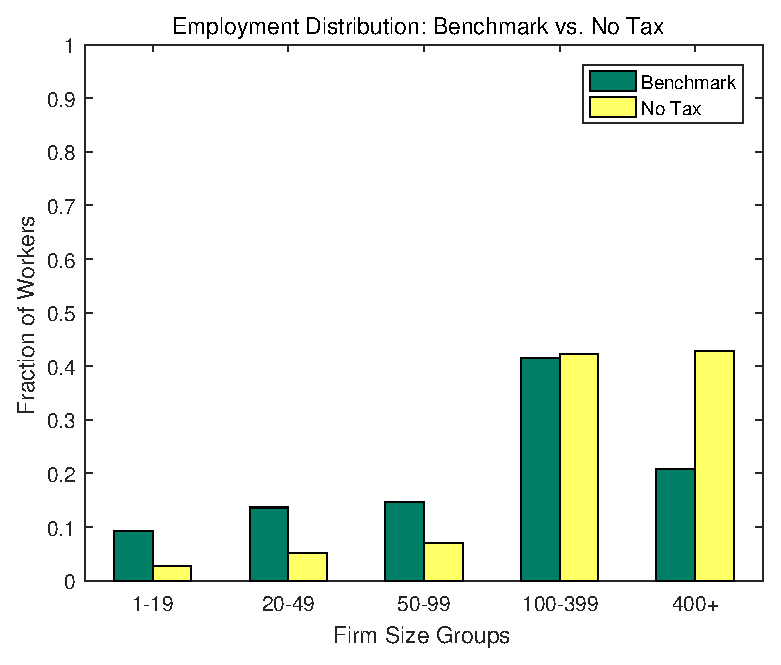
\includegraphics[width=0.45\textwidth]{./Figures/bench_notax_es.eps}
    \includegraphics[width=0.45\textwidth]{./Figures/bench_reg_es.eps}
    \caption{The Effects of Distortions and Regulations on Firm Size Distributions}
    \begin{figurenotes}
        The distributions of the polluting sector are reported.
    \end{figurenotes}
    \label{fig:compare_size}
    \end{center}
\end{figure}

The large increase in aggregate output is caused by both an improved allocation of production factors across firms, and a large increase in capital accumulation of about 60\% due to decrease in average tax rate from 13\% to 0\%. The increase in capital accumulation plays a much larger role than improved allocation of factors in the increase in aggregate output. Our quantitative exercise in Section IV.B below illustrates this point further. The large decline in average pollution intensity is also caused by two factors: the improved allocation of production factors, and increased adoption of the clean technology. After the removal of correlated distortions, more production factors move to large productive firms which also have lower pollution intensity. This reallocation lowers the average pollution intensity. Meanwhile, as we discuss in Section III.D, correlated distortions lower the elasticity of firm profits to firm TFP $z$, and therefore dampen their incentives to adopt the clean technology. Removing correlated distortions would do exactly the opposite and encourage the adoption of clean technology.

To evaluate the relative contributions of the improved allocation of factors and improved adoption of clean technologies, we consider a hypothetical economy that is identical to our benchmark economy, except that the clean technology shows no improvement in abatement efficiency over the dirty technology, that is, $\psi_0^{1} = \psi_0^{0}$ and $\psi_1^{1} = \psi_1^{0}$. First, we remove correlated distortions from this hypothetical economy, which reveals the importance of the improved allocation of factors. We then re-introduce the differences between clean and dirty technologies to the hypothetical economy, so that the resulting equilibrium is exactly the same as that in Experiment (i). The latter calculation reveals the importance of the improved adoption of clean technologies. We find that the improved adoption of clean technology accounts for 48\% of the decrease in average intensity.

Finally, the polluting and non-polluting sectors respond in similar ways to the removal of correlated distortions, and little reallocation is induced across sectors. Recall that the distributions of managerial talent and distortions are the same across these two sectors, and the only material difference between these two sectors is the presence of the fixed adoption cost of clean technology $k_E$ and environmental regulations in the polluting sector. Since the calibrated value of $k_E$ is not too large, the differences in the reaction of these two sectors to the removal of distortions are rather limited.

One notable difference is that the mean firm size is somewhat larger in the polluting sector, because environmental regulations work as an additional selection mechanism. The interaction between the correlated distortions and environmental regulations leads to further efficiency losses in the polluting sector, because average firm size and hence the effective distortions increase. As a result, compared to the non-polluting sector, the removal of correlated distortions leads to a 1.5 percentage points larger increase in output in the polluting sector.

\textit{Tightening Environmental Regulations.}---In Experiment (ii), we increase environmental penalties $\xi$ to the extent that the fraction of firms using the clean technology increases to the same 85\% as in Experiment (i). The results are shown in Column (ii) of Table \ref{tab:aggregates}. Overall, in the polluting sector, the increase in $\xi$ leads to small decreases in aggregate output, capital stock and equilibrium wage, a sizable change in firm size distribution, and substantial decreases in aggregate pollution and pollution intenisty. On the other hand, the increase in $\xi$ has very limited spillover on both the aggregate outcomes and firm size distribution to the non-polluting sector.

The increase in $\xi$ affects the resource allocation in the polluting sector along both the extensive and intensive margins. Most notable changes come along the extensive margin. In our model as well as in the data, it is the small unproductive firms that choose the dirty technology. Therefore, an increase in environmental penalties would mostly fall on small unproductive firms and lower their profits. This would drive a substantial fraction of small firms out of the market through the endogenous occupation choice, and lead to a sizable increase in average firm size. Meanwhile, labor supply increases as the managers of these exiting firms now choose to be workers, which suppresses the equilibrium wage. These changes along the extensive margin are efficiency-improving in the presence of correlated distortions, since the direction of the factor reallocation is opposite to that induced by the correlated distortions.

While small firms account for a large fraction of firms, they account for only a small fraction of production factors, which implies that the total amount of factors affected by the extensive margin is small. In addition, the polluting sector only account for 20\% of production factors in the benchmark economy. Therefore, the induced decline in equilibrium wage is very small (0.04\%). In addition, our calibrated value of the adoption cost of clean technology $k_E$ is not too large. Therefore, the impact on surviving firms in the polluting sector is also limited, which can be seen from Table \ref{tab:talentdist}. Despite this, the allocation of factors along the intensive margin worsens, in the sense that the share of factors used by the most productive group decreases, because more distorted productive firms benefit less from the wage decline. This offsets the improvement in efficiency from the reallocation along the extensive margin.

Since the total amount of factors involved in reallocation along the two margins is small, most of the decrease in average pollution intensity comes from the increased adoption of the clean technology. We repeat the same decomposition exercise as we did in Experiment (i), and find that 94\% and 96\% of the reductions in aggregate pollution and average intensity, respectively, stem from the increased adoption of the clean technology. Since the output of the polluting sector decreases only slightly in this experiment, the decreases in aggregate pollution and intensity are quantitatively similar at around 14\%.

The non-polluting sector is indirectly affected in this experiment by the general equilibrium response in wage. Since the induced change in equilibrium wage is very small, the increase in $\xi$ has very small effects on both the aggregate outcomes and firm size distribution, even when the products of the two sectors are perfect substitutes.

\textit{Comparing the Two Experiments.}---Both experiments cause the reallocation of factors across firms, but in different ways. Removing the correlated distortions from both sectors improve resource allocation along both the extensive and intensive margins, which push the economy closer to the production possibility frontiers. In contrast, while tightening environmental regulations leads to tougher selection of firms, which pushes the extensive margin closer to its first-best level, the resource allocation across firms along the intensive margin worsens.\footnote{In reality, tightening environmental regulations may cause other undesirable outcomes. For example, extra resources are needed to enforce tightening regulations, and more rent-seeking activities may possibly be induced by the regulations. Due to data limitations, we leave a complete welfare analysis of tightening environmental regulations to future research.} As a result, although the fraction of firms using clean technology is set to be the same in the two experiments, the reduction of aggregate pollution intensity is larger in Experiment (i), because the larger (and cleaner) firms take a much larger market share compared to Experiment (ii).

\subsection{Effects of the Progressivity of the Distortions}
\label{sec:progressivity}

In Experiment (i), by setting $\tau_z = 0$, we change both the progressivity and and the average level of distortions. To isolate the importance of the progressivity of $\tau_z$, we solve a version of the model where the progressive taxes are replaced with uniform taxes by setting $\phi_1 =$ 0, and change $\phi_0$ to keep the total implicit tax revenue constant.\footnote{This strategy has a long tradition in the public finance and development economics literature. See for example, \citet{Ventura:1999}, \citet{ConesaKrueger:2006}, \citet{Bhattacharyaetal:2013} and \citet{BentoRestuccia:2016}, among others.} Not surprisingly, the implied uniform tax rate $\tau_z =$ 18\% is higher than the average tax rate of 13\% under the progressive tax system. Column (i') in Table \ref{tab:uniform} summarizes the results from this experiment and compares them to those from Experiment (i). A comparison of Column Benchmark and Column (i') reveals the effects of a change in progressivity of $\tau_z$, while a comparison of Column (i') and (i) highlights the effects of a uniform change in tax rates across firms.

\begin{table}[t]
\footnotesize
\centering
\caption{The Effects of the Progressivity of Distortions}
\begin{tabular}{lccccccc}
    \hline \hline
                         & \multicolumn{3}{c}{Polluting}    & & \multicolumn{3}{c}{Non-polluting} \\
    \cmidrule{2-4} \cmidrule{6-8}
    Statistics           & Benchmark & (i')      & (i)      & & Benchmark     & (i')    & (i) \\
    \hline
    Output               & 100.00    & 108.15   & 131.16    & & 100.00        & 106.87 & 129.62 \\
    Capital              & 100.00    & 110.91   & 163.06    & & 100.00        & 109.63 & 161.26 \\
    Consumption          & 100.00    & 106.57   & 123.63    & & 100.00        & 106.57 & 123.63 \\
    Wage                 & 100.00    & 108.76   & 160.00    & & 100.00        & 108.76 & 160.00 \\
    Output per Worker    & 100.00    & 105.74   & 128.25    & & 100.00        & 106.03 & 128.60 \\
    \hline
    \# of Firms          & 100.00    & 44.07    &44.07      & & 100.00        & 41.56  & 41.56 \\
    Mean Size            & 59.98     & 139.19   & 139.19    & & 52.18         & 126.53 & 126.53 \\
    \hline
    Pollution            & 100       & 70.04    & 76.67     \\
    Intensity            & 100       & 64.78    & 58.46     \\
    Clean Share          & 57.77     & 73.33    & 85.61     \\
    \hline
\end{tabular}
\begin{tablenotes}
     All of the values are percentages except for mean firm size, which are the numbers of workers. Consumption and wage are not sector specific.
\end{tablenotes}
\label{tab:uniform}
\end{table}

As we can see from Table \ref{tab:uniform}, removing the progressiveness of $\tau_z$ increases aggregate output, capital, consumption and output per worker. However, the 6\% to 11\% increases here are rather moderate compared to the 20\% to 60\% increases when all the distortions are eliminated. These differences are mainly caused by the relatively high level of the uniform tax rate of 18\% in Experiment (i'), which discourages capital accumulation and results in much lower capital stock compared to the case of $\tau_z =$ 0.\footnote{Our results on aggregate output also appear rather moderate compared to those in \citet{RestucciaRogerson:2008}, who control for the capital accumulation effects in their quantitative exercises. This is mainly because that the distortions in their paper cause large rank reversals between firm TFP and size, while the distortions in our paper preserve ranks. Please see the related discussions in \citet{Hopenhayn:2014}.}

However, removing the progressiveness of $\tau_z$ causes a large change in firm size distribution, and therefore large declines in aggregate pollution and pollution intensity. In fact, the resulting number of firms and mean firm size are the same between Experiment (i) and (i'), since the only difference between them is a uniform increase in tax rates across firms. The average pollution intensity decreases by 35\% when the progressiveness of $\tau_z$ is removed, compared to a 42\% decline when all the correlated distortions are eliminated. Again, the decline in average pollution intensity is caused by both an improved resource allocation and improved adoption of the clean technology among firms. However, the second channel is not as strong as in Experiment (i) (16 versus 28 percentage points), since the increases in firm's profit are not as large as in Experiment (i). Moreover, since the output of the polluting sector only increases by 8\% in this experiment compared to 30\% in Experiment (i), the 30\% decline in aggregate pollution here is larger than the 23\% in Experiment (i).

In sum, our findings imply that it is the progressiveness of firm-level distortions, rather than the average level of distortions, that plays a dominate role in amplifying aggregate pollution and pollution intensity.

\section{Conclusions}

This paper proposes a novel explanation for the industrial water pollution problem in China. In our theory, large productive firms are more likely to use the clean technology and have lower pollution intensity, largely due to the fixed adoption cost of clean technology and imperfect environmental regulations. Distortions that increase with firm TFP reallocate production factors away from large productive firms, therefore reduce aggregate output while increasing aggregate pollution intensity. We support our theory by firm-level data on production, emissions and pollution treatment technologies from China. Quantitatively, we find that distortions correlated with firm TFP reduce aggregate output by about 30\% and increase aggregate pollution by about 20\%.

Our findings have novel implications for both resource misallocation and environmental pollution. They imply that the welfare losses from misallocation include not only lower economic output, which is the focus of previous studies, and but also more pollution. This could have important welfare consequences given the severity of pollution in China and other developing countries. Our findings also challenge a popular view that economic growth necessarily comes at the cost of more pollution in developing countries. They suggest that a growth path with both higher output and lower pollution is attainable, if policy and institutional distortions can be removed in a cost-effective way.

The analytical framework in this paper can be extended to other pollutants, sectors and countries. For other pollutants, China also has a severe air pollution problem, and casual observations reveal that small and medium-sized firms in high-polluting industries such as steel contribute disproportionately to air pollution in China as well. For other sectors, \citet{AGpaper} find that misallocation caused by migration and land policies is an important driver of agricultural pollution in China. For other countries, \citet{HsiehKlenow:2014} and \citet{BentoRestuccia:2016} find evidence of distortions that are highly correlated with firm TFP in a number of developing countries, while \citet{Dasguptaetal:1998} find that small firms have higher air pollution intensity in Brazil and Mexico. It would be interesting to assess the impact of distortions on pollution in these countries.

\bibliographystyle{aea}
\bibliography{./Dissertation1}

\end{document}

